\documentclass[10pt,a4paper]{article}

\usepackage[utf8x]{inputenc}
\usepackage{ucs}
\usepackage[francais]{babel}
\usepackage[T1]{fontenc}

\usepackage{amsmath}
\usepackage{amsfonts}
\usepackage{amssymb}

\usepackage{graphicx}

\usepackage{boxedminipage}
\addtolength{\fboxsep}{3pt}

\title{Cahier des charges de Bob-Project}
\author{LAFON Sylvain, LEVASSEUR Thomas et MAINGRET François}

\begin{document}
	\maketitle
	\tableofcontents
	\newpage
	\part{Introduction}
		Le bricolage et le jardinage etants à la mode des derniers temps, le site Brico-Bob vise à proposer à des utilisateurs de profils variés, aussi bien
la ménagère que le retraité ou que les jeunes couples, du matériel à la vente ou à la location.
Ce site étant de nature commerciale, il se doit d'etre visuellement attractif et d'etre ergonomique. La présentation des produits devra etre simple, claire, et 
bien organisée, l'utilisateur devra pouvoir trouver un produit le plus rapidement possible afin qu'il ne se lasse pas du site et qu'il achète le plus de prosuits
possible ( De plus, il existera une fonction pour rechercher un produit selon differents critères. De la publicité sur certaines pages du site pourra influencer
le client.
Chaque utilisateur du site devra s'inscrire en fournissant un login et un mot de passe pour  faire ses achats, ses informations personnelles ( nom, adresse... )
ne seront demandées que lors de la validation de la commande ). Chaque membre du site pourra poster des avis, et noter les differents produits, ainsi que poser
des questions techniques.
Enfin, l'administrateur du site pourra gerer simplement, depuis une fenetre speciale, le contenu du magasin, et les membres.

	\newpage
	\part{Fonctionnalités}
		\section{Cas d'utilisation}
			\subsection{Description des acteurs}
				Il existe 3 acteurs principaux au sein de cette application :

\subsubsection{internaute} 

l'internaute est un visiteur de passage, qui peut venir pour la premiere fois sur le site, pour rechercher et consulter des produits, par exemple pour comparer
les prix avec la concurence. il peut également etre un visiteur regulier qui verifie les promotions en cours. bien que cet internaute puisse accèder a une grande partie des pages du site, ses possibilités sont limités, il a donc la posibilité de s'inscrire afin de devenir membre

\subsubsection{membre}

le membre est un internaute qui s'est inscrit au site, en ne donnant aucune information personnelle, apart son e-mail, necessaire en cas de problème. 
il aura la possibilité de poser des questions sur des produits, de donner son avis ainsi que de noter les articles, mais surtout d'acheter ou de louer des produits.
Le membre ne fournirra ses coordonnées que lors de sa premiere commande, ce pour lui demander les informations necessaires en temps voulu, qu'il ne fournisse pas son nom alors que ce n'est pas encore nesessaire, pour des questions de protection de la vie privée.

\subsubsection{admin}

les administrateurs du site pourront faire tout ce que les membres peuvent faire, mais auront accès a un panneau d'administration, que nous verrons en details plus tard dans ce dossier, qui leur permettra de gerer tout le contenu du site ainsi que les membres, sans passer directement pas le SGBD, ce qui est plus simple d'utilisation (un admin pourra ajouter des produits, promotions, bannir un membre... voir user case  ).
Toutefois, l'administateur ne pourra pas modifier un message ecrit pas un membre, ni les informations sur un membre.

			\subsection{Diagramme de cas d'utilisation}
				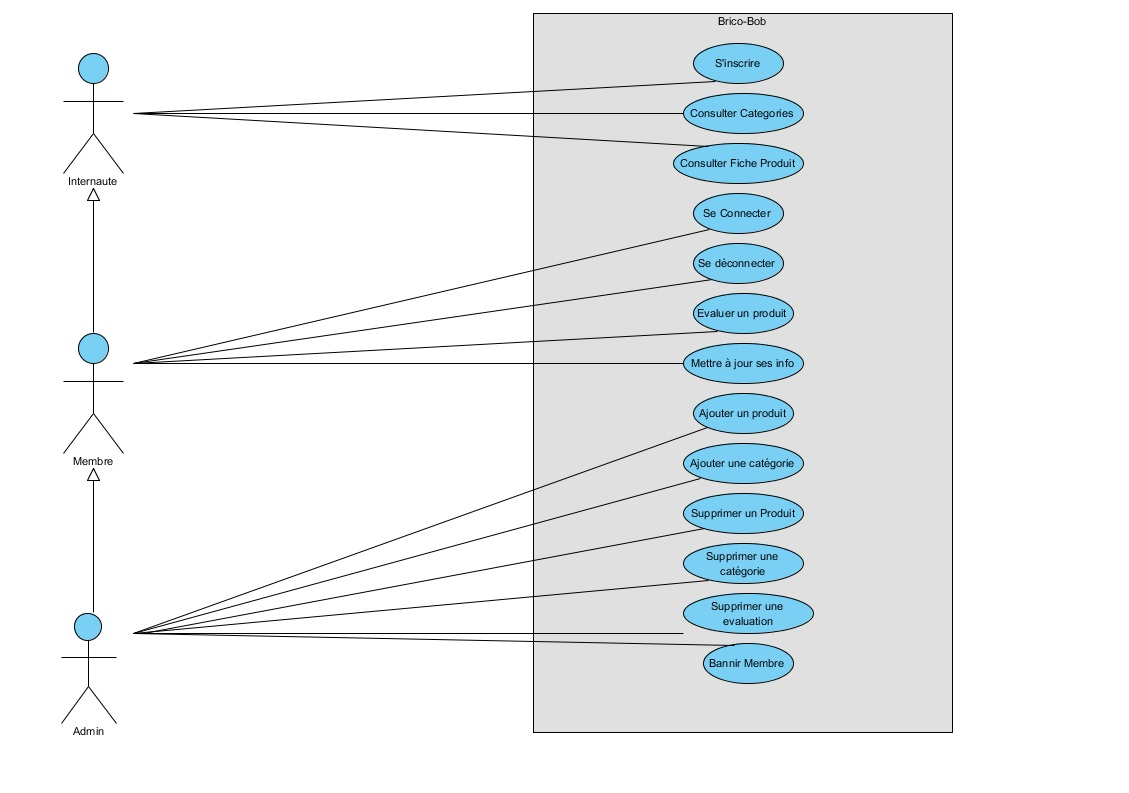
\includegraphics[scale=0.7,angle=270]{cas/diagramme.jpg}
			\subsection{Scénario de cas d'utilisation}
				\subsubsection{Inscription, connexion et deconnexion}
					1 Le système propose à l'internaute de s'inscrire.
2 L'internaute clique sur "s'inscrire".
3 Le système demande à l'internaute de lui fournir un nom de compte, un mot de passe et une vérification du mot de passe.
4 L'internet entre les informations demandées.
5 L'internaute clique sur "s'inscrire".
6 L'internaute est inscrit et connecter.

Exceptions: 
			5a L'internaute a entrer un pseudo éxistant.
			6 Le systeme affiche "Pseudo déja utiliser".
			7 Le système propose de nouveau à l'internaute de s'incrire.
			
			5a L'internaute a entrer deux mot de passe differents.
			6 Le système affiche "Les mots de passe ne sont pas identiques".
			7 Le système propose de rentrer à nouveau les mots de passe.

\begin{boxedminipage}[t]{12cm}
	\begin{itemize}
		\item Système : Site web "Chez Bob"
		\item Acteur : Internaute
		\item Objectif : Inscrire un compte
		\item Pré-condition : (aucune)
	\end{itemize}

	\renewcommand\theenumi{\arabic{enumi}}
	\renewcommand\labelenumi{\theenumi .}
	\renewcommand\theenumii{\Alph{enumii}}
	\renewcommand\labelenumii{(\theenumii)}
	\paragraph{Scénario :} 
	\begin{enumerate}
		\item \label{sc1l1} un item
	\end{enumerate}
\end{boxedminipage}
\newpage

\begin{boxedminipage}[t]{12cm}
	\begin{itemize}
		\item Système : Site web "Chez Bob"
		\item Acteur : Internaute
		\item Objectif : Se connecter sur le compte de l'utilisateur
		\item Pré-condition : L'utilisateur est enregistré
	\end{itemize}

	\renewcommand\theenumi{\arabic{enumi}}
	\renewcommand\labelenumi{\theenumi .}
	\renewcommand\theenumii{\Alph{enumii}}
	\renewcommand\labelenumii{(\theenumii)}
	\paragraph{Scénario : }
	\begin{enumerate}
		\item \label{sc2l1} Le système propose à l'utilisateur de se connecter à son compte.
		\item \label{sc2l2} L'utilisateur clique sur "se connecter".
		\item \label{sc2l3} Le système demande le nom de compte et le mot de passe de l'utilisateur.
		\item \label{sc2l4} L'internaute entre les informations demandées.
		\item \label{sc2l5} L'internaute clique sur "se connecter".
		\item \label{sc2l6} L'internaute est connecté à son compte.
	\end{enumerate}

	\renewcommand\theenumi{\Alph{enumi}}
	\renewcommand\labelenumi{\theenumi )}
	\renewcommand\theenumii{\arabic{enumii}}
	\renewcommand\labelenumii{\theenumii .}
	\paragraph{Exceptions :} 
	\begin{enumerate}
		\item
		\begin{enumerate}
			\addtocounter{enumii}{4}
			\item Une des informations ou les deux demandées ne correspondent pas.
			\item Le système affiche un message d'erreur
			\item Retour à \ref{sc2l3}
		\end{enumerate}
	\end{enumerate}
\end{boxedminipage}
\newline

\begin{boxedminipage}[t]{12cm}
	\begin{itemize}
		\item Système : Site web "Chez Bob"
		\item Acteur : Internaute
		\item Objectif : Se déconnecter de son compte
		\item Pré-condition : L'utilisateur est connecté à son compte
	\end{itemize}

	\renewcommand\theenumi{\arabic{enumi}}
	\renewcommand\labelenumi{\theenumi .}
	\renewcommand\theenumii{\Alph{enumii}}
	\renewcommand\labelenumii{(\theenumii)}
	\paragraph{Scénario :} 
	\begin{enumerate}
		\item \label{sc3l1} Le système propose à l'utilisateur de se déconnecter de son compte.
		\item \label{sc3l2} L'utilisateur clique sur "se déconnecter".
		\item \label{sc3l3} Le système déconnecte le membre de son compte.
		\item \label{sc3l4} Le système redirige l'internaute vers l'accueil.
	\end{enumerate}
\end{boxedminipage}
\newpage

% On remet les valeurs qui sont là par défaut.
\renewcommand\theenumi{\arabic{enumi}}
\renewcommand\labelenumi{\theenumi .}
\renewcommand\theenumii{\Alph{enumii}}
\renewcommand\labelenumii{(\theenumii)}
				\subsubsection{Recherche d'un produit}
					%
%  Contient les 3 scénarios pour la recherche
%
\begin{boxedminipage}[t]{12cm}
	\begin{itemize}
		\item Système : Bob-Project
		\item Acteur primaire : internaute
		\item Objectif : Rechercher un produit (via la barre)
		\item Préconditions : (aucune)
	\end{itemize}

	\renewcommand\theenumi{\arabic{enumi}}
	\renewcommand\labelenumi{\theenumi .}
	\renewcommand\theenumii{\Alph{enumii}}
	\renewcommand\labelenumii{(\theenumii)}
	\paragraph*{Scénario 1 :}
	\begin{enumerate}
		\item \label{sr1l1} L'utilisateur entre un nom de produit à rechercher
		\item \label{sr1l2} Le système recherche tout d'abord le nom exact
		\item \label{sr1l3} Le système recherche ensuite les noms qui ressemblent
		\item \label{sr1l4} Le système affiche une page de résultat dans laquelle on trouve les différents produits.
	\end{enumerate}


	\renewcommand\theenumi{\Alph{enumi}}
	\renewcommand\labelenumi{\theenumi )}
	\renewcommand\theenumii{\arabic{enumii}}
	\renewcommand\labelenumii{\theenumii .}
	\paragraph*{Exceptions :}
	\begin{enumerate}
		\item
			\begin{enumerate}
				\item L'utilisateur valide en ayant laissé un champ vide
				\item Le système renvoie l'utilisateur vers la page de Recherche avancée en lui disant que le champ n'était pas rempli
			\end{enumerate}
		\item
			\begin{enumerate}
				\addtocounter{enumii}{1}
				\item Le système ne trouve aucun résultat
				\item Le système recherche ensuite les noms qui ressemblent
				\item Le système affiche une page de résultat dans laquelle on trouve les produits avec un nom ressemblant, et propose une correction de la recherche.
			\end{enumerate} 
		\item
			\begin{enumerate}
				\addtocounter{enumii}{2}
				\item Le système ne trouve aucun résultat
				\item Le système renvoie l'utilisateur vers la page de Recherche avancée en lui disant que rien n'à pu être trouvé
			\end{enumerate}
		\item
			\begin{enumerate}
				\addtocounter{enumii}{1}
				\item Le système trouve beaucoup de résultats
				\item Le système affiche une page de résultat dans laquelle on trouve les différents produits avec un message comme quoi une recherche avancée pourrait affiner le résultat.
			\end{enumerate}	
	\end{enumerate}
\end{boxedminipage}
\newpage
\begin{boxedminipage}[t]{12cm}
	\begin{itemize}
		\item Système : Bob-Project
		\item Acteur primaire : internaute
		\item Objectif : Rechercher un produit (via la page de Recherche avancée)
		\item Préconditions : être en train d'aller sur la page (redirection ou lien)
	\end{itemize}

	\renewcommand\theenumi{\arabic{enumi}}
	\renewcommand\labelenumi{\theenumi .}
	\renewcommand\theenumii{\Alph{enumii}}
	\renewcommand\labelenumii{(\theenumii)}
	\paragraph*{Scénario 2 :}
	\begin{enumerate}
		\item \label{sr2l1} Le système présente un grand formulaire contenant notemment :
			\begin{itemize}
				\item Nom du produit (*)
				\item Catégorie du produit
				\item Prix du produit
				\item (autres critères comme la marque)
			\end{itemize}
		\item \label{sr2l2} Le système lance la recherche avec la recherche exacte
		\item \label{sr2l3} Le système lance la recherche sur le nom
		\item \label{sr2l4} Le système lance la recherche sur les produits qui ont des points communs
		\item \label{sr2l5} Le système affiche une page de résultat avec le resultat du \ref{sr2l2} visible et demande si les autres résultats peuvent être affichés
	\end{enumerate}

	\renewcommand\theenumi{\Alph{enumi}}
	\renewcommand\labelenumi{\theenumi )}
	\renewcommand\theenumii{\arabic{enumii}}
	\renewcommand\labelenumii{\theenumii .}
	\paragraph*{Exceptions :}
	\begin{enumerate}
		\item
			\begin{enumerate}
				\item L'utilisateur ne rentre pas le nom du produit (obligatoire)
				\item Le système affiche un message d'erreur
				\item Retour à \ref{sr2l1}
			\end{enumerate}
		\item
			\begin{enumerate}
				\addtocounter{enumii}{3}
				\item Vraiment aucun résultat
				\item Le système envoie un message d'excuse : aucun produit n'a pu être trouvé
				\item Retour à \ref{sr2l1}
			\end{enumerate}
	\end{enumerate}
\end{boxedminipage}
\newpage
\begin{boxedminipage}[t]{12cm}
	\begin{itemize}
		\item Système : Bob-Project
		\item Acteur primaire : internaute
		\item Objectif : Rechercher un produit (via l'exploration)
		\item Préconditions : (aucune)
	\end{itemize}

	\renewcommand\theenumi{\arabic{enumi}}
	\renewcommand\labelenumi{\theenumi .}
	\renewcommand\theenumii{\Alph{enumii}}
	\renewcommand\labelenumii{(\theenumii)}
	\paragraph*{Scénario 3 :}
	\begin{enumerate}
		\item \label{sr3l1} L'utilisateur passe la souris sur Acheter ou Louer (menu)
		\item \label{sr3l2} L'utilisateur clique sur une catégorie
		\item \label{sr3l3} Le système affiche la page de la sous-catégorie
		\item \label{sr3l4} L'utilisateur clique sur un produit
		\item \label{sr3l5} (L'utilisateur à trouvé son produit)
	\end{enumerate}

	\renewcommand\theenumi{\Alph{enumi}}
	\renewcommand\labelenumi{\theenumi )}
	\renewcommand\theenumii{\arabic{enumii}}
	\renewcommand\labelenumii{\theenumii .}
	\paragraph*{Exceptions :}
	\begin{enumerate}
		\item
			\begin{enumerate}
				\item L'utilisateur clique sur Acheter ou Louer
				\item Le système affiche la page des catégories
				\item Retour à \ref{sr3l2}
			\end{enumerate}
		\item
			\begin{enumerate}
				\addtocounter{enumii}{3}
				\item L'utilisateur clique sur une autre sous-catégorie
				\item Retour à \ref{sr3l3}
			\end{enumerate}
		\item
			\begin{enumerate}
				\addtocounter{enumii}{4}
				\item (L'utilisateur ne trouve pas son produit)
				\item Rien ne se passe : il peut continuer à explorer ou bien passer à autre chose ou encore utiliser la barre de recherche
			\end{enumerate}
	\end{enumerate}
\end{boxedminipage}
\newpage

\renewcommand\theenumi{\arabic{enumi}}
\renewcommand\labelenumi{\theenumi .}
\renewcommand\theenumii{\Alph{enumii}}
\renewcommand\labelenumii{(\theenumii)}
				\subsubsection{Affichage d'un produit}
					\begin{boxedminipage}[t]{12cm}
  \begin{itemize}
		\item Système : Site web "Chez Bob"
		\item Acteur : Internaute
		\item Objectif : Visualiser Fiche Produit
		\item Pré-condition : L'utilisateur à trouvé un produit ou une liste de produits
	\end{itemize}

	\paragraph{Scénario : }
	\begin{enumerate}
		\item \label{sll1} Le système propose à l'utilisateur un ou plusieurs produits a visualiser.
		\item \label{sll2} L'utilisateur sélectionne le produit qu'il souhaite visualiser
		\item \label{sll3} Le système recherche les info relatives au produit dans la DB
		\item \label{sll4} Le système affiche les informations relatives au produit ( Nom, prix, description, photo, note, commentaires... )
	\end{enumerate}

\newline
\end{document}